
\section{Push-Pull Block Puzzles}
In this section we prove several results about push-pull block puzzles. We show Push-$1$ Pull-$1$ in 3D with thin walls is PSPACE-complete in Section~\ref{3DPSPACE}; Push-$i$ Pull-$j$ in 3D is PSPACE-complete for all positive integers $i,j \geq 2$ in Section~\ref{3DPSPACE}; Push-$k$ Pull-$l$ in 3D is NP-hard for all positive integers $k, l$ in Section~\ref{3DNPhard}; and Push-$q$ Pull-$r$ in 2D with thin walls is NP-hard for all positive integers $q$, $r$ in Section~\ref{2DNPhard}. A summary of these results can be seen in Table~\ref{BlocksTable}.


\subsection{2D Push-Pull with Thin Walls}
\label{2DNPhard}
In this section we prove that Push-$k$ Pull-$l$ in 2D with fixed blocks is NP-hard, for all positive $k$ and $l$, if we include \emph{thin walls}. Thin walls are a new, but natural, notion for block pushing puzzles. They prevent blocks or the robot from passing between two adjacent, empty squares, as though there were a thin wall blocking the path. We will prove hardness by a reduction from 3SAT. The 3SAT problem asks whether, given a set of variables $\{x_1, x_2, \ldots x_n\}$ and a boolean formula in conjunctive normal form with exactly three variables per clause, there exists an assignment of values to those variables that satisfies the formula.\cite{NPBook} To do so we will introduce an abstract gadget called the Set-Verify gadget.

\begin{theorem}
\label{thm:2DNPhard}
Push-$k$ Pull-$l$ in 2D with thin walls is NP-hard.
\end{theorem}

\subsection{3SAT Construction}
\label{sec:2DPushPull3SAT}

We will be making use of the Set-Verify gadget to produce the literals in our 3SAT formula. One significant difficulty with this model is the complete reversibility of all actions. Thus we need to take care to ensure that going backward at any point does not allow the robot to cheat in solving our 3SAT instance. The directional properties of the Set-Verify allow us to create sections where we know if the robot exits, it must have either reset everything to the initial configuration or put everything in another known state.

Our literals will be represented by Set-Verify gadgets, described in Section~\ref{sec:SetVerifyGadgets}. They are considered true when the $V_i$ to $V_o$ traversal is possible, and false otherwise. Thus we can set literals to true by allowing the robot to run through the $S_i$ to $S_o$ passage of the gadget. This allows a simple clause gadget, shown in Figure~\ref{fig:NPClauseGadget}, consisting of splitting the path into three hallways, each with the corresponding verify side of our literal. We can then pass through if any of the literals are set to true, and cannot pass otherwise.

The variables will be encoded by a series of passages which split to allow either the true or negated literals to be set, shown in Figure~\ref{fig:NPVariableGadget}. Once variables split into two hallways, we have to show that when it enters or exits a side of a hallway, all the literals are set to true at one end and false at the other. Also, we cannot go back through the other hallway, so if we go backward, everything gets reset. Thus we cannot exploit the reversibility to set anything extra true.

The variables and clauses must be joined together to allow the robot to move between the gadgets in the correct order. We can connect these with simple, empty hallways, except in the cases where these hallways must cross. To deal with this we construct crossover gadgets from the Set-Verify gadgets. In order to traverse all of the clauses and reach the goal location, the robot must traverse a set of variable hallways that encode an accepting assignment to the 3SAT problem, thus reducing 3SAT to 2D Push-Pull block puzzles.


\begin{figure}[!ht]
\begin{minipage}{.36\textwidth}
    \includegraphics[width=\textwidth]{NPClauseGadget}
    \caption{Clause gadget, $C_k$, with variables $x_a$, $x_b$, $x_c$.}
    \label{fig:NPClauseGadget}
\end{minipage}
\hspace{5mm}
\begin{minipage}{.57\textwidth}
  \centering
    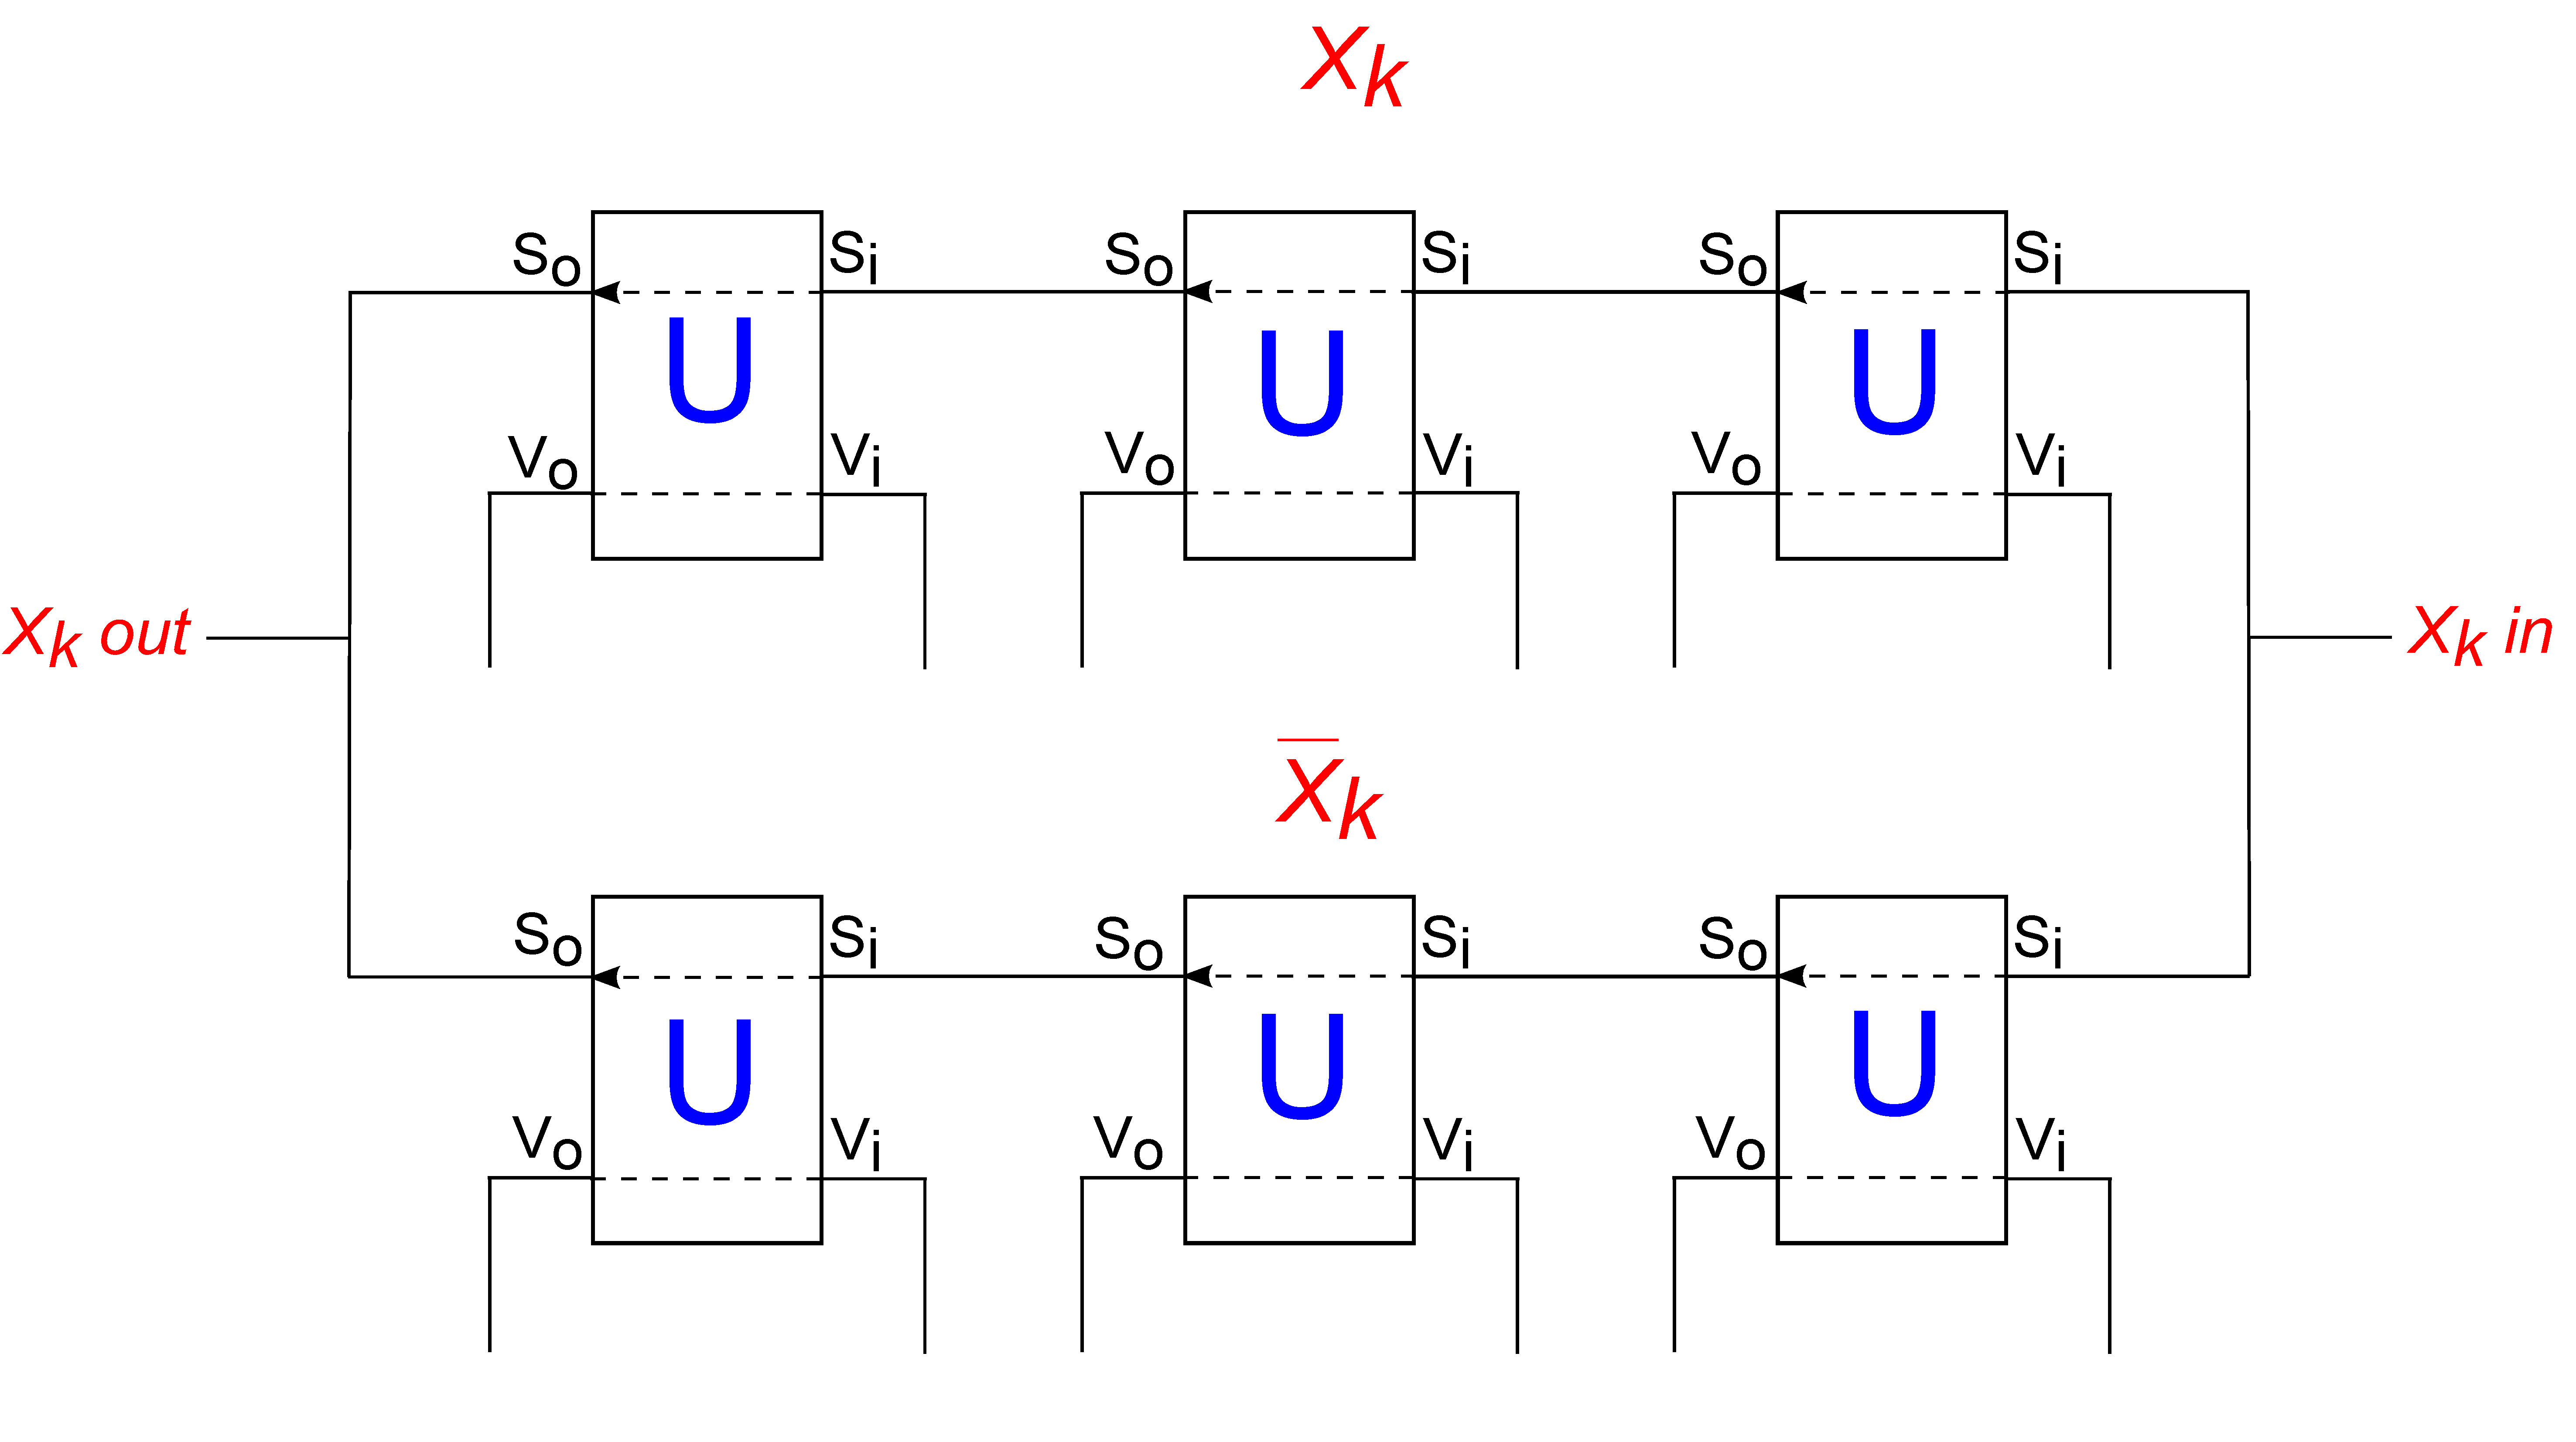
\includegraphics[width=.8\textwidth]{NPVariableGadget}
    \caption{A variable gadget representing $X_k$ occurring in six clauses.}
    \label{fig:NPVariableGadget}
\end{minipage}
\end{figure}

%\xxx{consider reviving one-way gadget (actually a 1-toggle)}
%\section{Reversible One-Way Gadget}
%When in the initial configuration $A$ the gadget only permits a traversal from $S_o$ to $S_i$ leaving the gadget in configuration $B$. Configuration $B$ only permits traversals in the opposite direction, from $S_i$ to $S_o$. Note, when the robot leave this gadget, the only possible configurations are $A$ and $B$. These gadgets or similar structures will be used several times within more complicated structures.
%
%\begin{figure}[!ht]
%  \centering
%    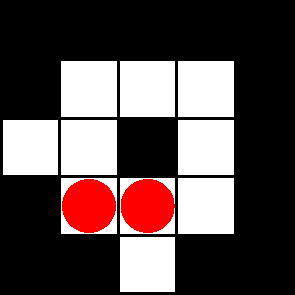
\includegraphics[width=0.8\textwidth]{one_way.pdf}
%    \caption{Reversible one-way gadget.}
%    \label{ldeScreenshotsMap}
%\end{figure}
\subsubsection{Set-Verify Gadgets}
\label{sec:SetVerifyGadgets}
There are four possible states of the Set-Verify gadget: Broken, Unset, Set, and Verified. The three relevant states are depicted in Figure~\ref{setVerifyDiagrams}. In the Broken state, the only possible transition is $S_o \rightarrow S_i$, changing the state to Unset. This state can only be reached from Unset, and allows strictly less future transitions than Set, which can also be reached from Unset, so we will disregard it. In the Unset state, the $S_i \rightarrow S_o$ transition is the only possibility, changing the state to Set. In the Set state, the $S_o \rightarrow S_i$ transition is possible, changing the state back to Unset, as well as the $V_i \rightarrow V_o$ transition, which changes the state to Verified. Finally, from the Verified state, the only transitions possible are $V_o \rightarrow V_i$, changing the state back to Set, and $V_i \rightarrow V_o$, leaving the state as Verified.

For the Set-Verify gadget in the Unset state, the $S_i$ entrance is the only one which allows the robot to move any blocks. From the $S_i$ entrance they can traverse to $S_o$, and they can also pull the middle block down behind them. Doing so will allow a traversal from $V_i$ to $V_o$. To traverse back from $S_o$ to $S_i$, the robot must first traverse back from $V_o$ to $V_i$. Then, when the robot travels back from $S_o$ to $S_i$, they must push the middle block back, ensuring the $V_i$ to $V_o$ traversal is impossible. Further, access to any sequence of entrances will not allow the robot to alter the system to allow traversals between the $V_i$ and $S_i$ entrances. 

Since the Set-Verify gadget has no hallways with length greater than 3, any capabilities the robot may have of pushing or pulling more than one block at a time are irrelevant. Thus, the following proof will apply for all positive values of $j$ and $k$ in Push-$j$ Pull-$k$.

%\begin{figure}[!ht]
%  \centering
%  \caption{Set-Verify Gadgets}
%  \begin{subfigure}[b]{0.3\textwidth}
%    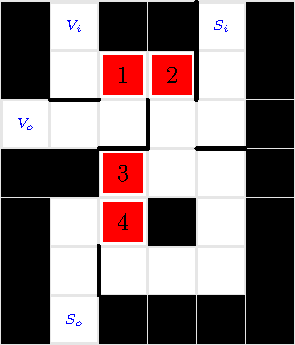
\includegraphics[width=\textwidth]{SetVerifyUnset}
%    \caption{Set-Verify, unset state.}
%    \label{SetVerifyUnset}
%  \end{subfigure}
%
%  \begin{subfigure}[b]{0.3\textwidth}
%    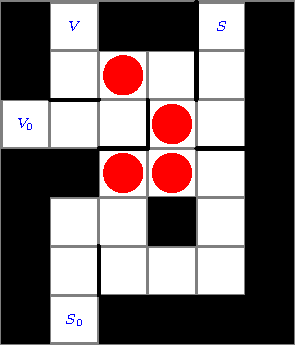
\includegraphics[width=\textwidth]{SetVerifySet}
%    \caption{Set-Verify, set state.}
%    \label{SetVerifySet}
%  \end{subfigure}
%  \begin{subfigure}[b]{0.3\textwidth}
%    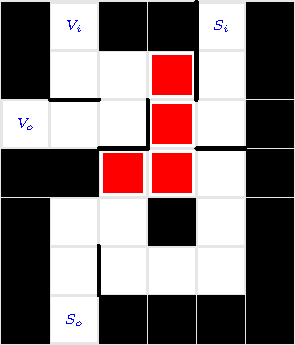
\includegraphics[width=\textwidth]{SetVerifyVerified}
%    \caption{Set-Verify, verified state.}
%    \label{SetVerifyVerified}
%  \end{subfigure}
%  \label{setVerifyDiagrams}
%\end{figure}

\begin{figure}[!ht]
  \centering
    \begin{subfigure}[b]{0.3\textwidth}
    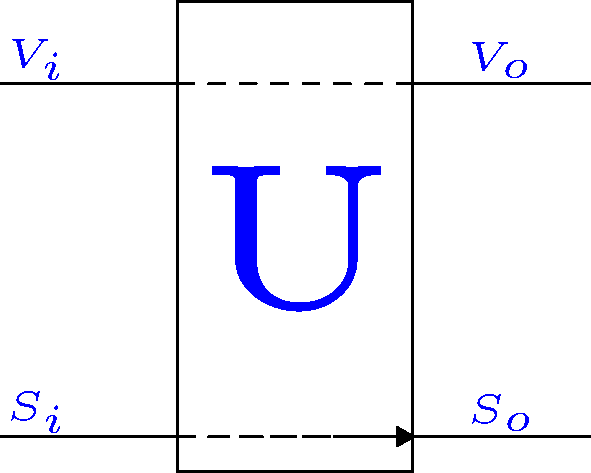
\includegraphics[width=\textwidth]{AbstractSetVerifyUnset}
    \caption{Abstract Unset Set-Verify}
    \vspace{15pt}
    \end{subfigure}
    \hfill
    \begin{subfigure}[b]{0.3\textwidth}
    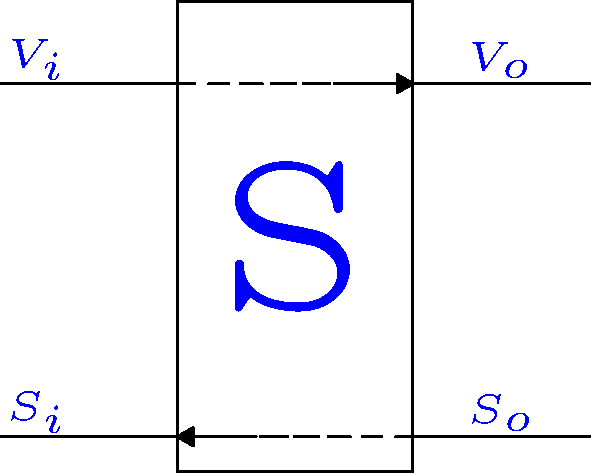
\includegraphics[width=\textwidth]{AbstractSetVerifySet}
    \caption{Abstract Set Set-Verify}
    \vspace{15pt}
    \end{subfigure}
    \hfill
    \begin{subfigure}[b]{0.3\textwidth}
    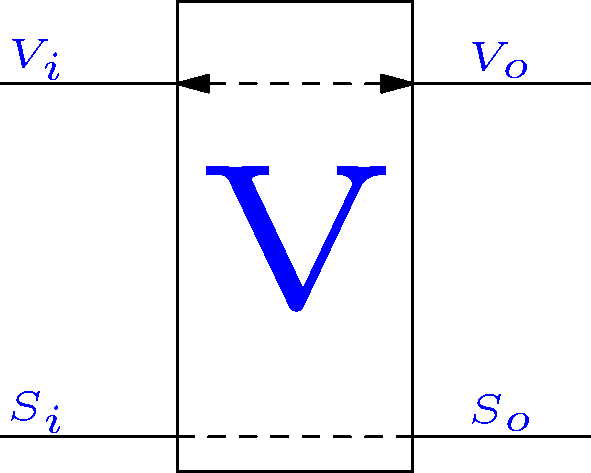
\includegraphics[width=\textwidth]{AbstractSetVerifyVerified}
    \caption{Abstract Verified Set-Verify}
    \vspace{15pt}
  \end{subfigure}  
   \vspace{10pt}
  \begin{subfigure}[b]{0.3\textwidth}
    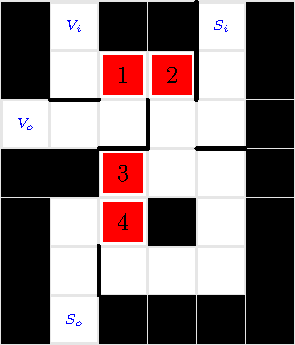
\includegraphics[width=\textwidth]{SetVerifyUnset}
    \caption{Set-Verify, unset state}
    \label{SetVerifyUnset}
  \end{subfigure}
  \hfill
  \begin{subfigure}[b]{0.3\textwidth}
    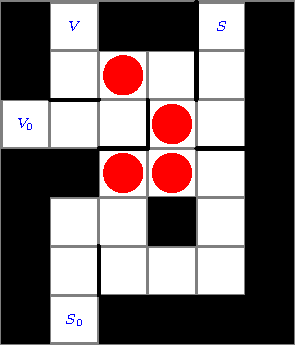
\includegraphics[width=\textwidth]{SetVerifySet}
    \caption{Set-Verify, set state}
    \label{SetVerifySet}
  \end{subfigure}
  \hfill
  \begin{subfigure}[b]{0.3\textwidth}
    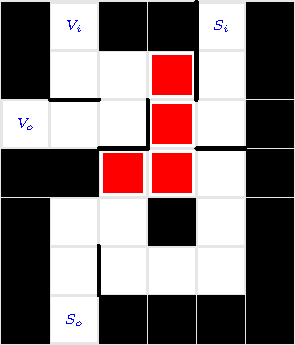
\includegraphics[width=\textwidth]{SetVerifyVerified}
    \caption{Set-Verify, verified state}
    \label{SetVerifyVerified}
  \end{subfigure}
  \caption{Set-Verify Gadgets}
  \label{setVerifyDiagrams}
\end{figure}

\subsubsection{Crossover Gadgets}
In this section we build up the needed one use crossover gadget from a series of weaker types of crossover gadgets.

\paragraph{Directed Destructive Crossover} This gadget, depicted in Figure~\ref{DestructiveCrossover}, allows either a traversal from $a$ to $a'$ or $b$ to $b'$. Once a traversal has occurred, that path may be traversed in reverse, but the other is impassable unless the original traversal is undone.

First, observe that transitions are initially only possible via the $a$ and $b$ entrances, since the transitions possible through a Set-Verify in the Set state can be entered through $V_i$ and $S_o$, not $S_i$. Assume without loss of generality that the gadget is entered at $a$. This changes the state of the left Set-Verify to Unset. At this point, only the right $V_i$ and left $S_i$ transitions are passable. Taking the $S_i$ transition reverts all changes to the original state. Taking the $V_i$ transition changes the right Set-Verify to Verified, and completes the crossover. At this point, the only possible transition is to undo the transition just made, from $a'$ back to $a$, restoring the original state. Thus, the only transition possibilities are as stated above.

\begin{figure}[!ht]
  \centering
  \begin{subfigure}[b]{0.47\textwidth}
    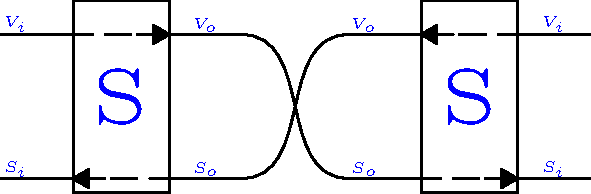
\includegraphics[width=\textwidth]{OneWayDestructiveCrossover}
    \caption{The one-way destructive crossover constructed from two connected Set-Verify gadgets initialized in the set position.}
    \label{DestructiveCrossover}
  \end{subfigure}
  \hfill
  \begin{subfigure}[b]{0.47\textwidth}
    \includegraphics[width=\textwidth]{InOrderCrossover}
    \caption{The in-order one-way crossover constructed from two connected Set-Verify gadgets initialized in the verified and unset positions.}
    \label{InOrderCrossover}
  \end{subfigure}
  \caption{Two types of crossover gadgets}
\end{figure}

\begin{figure}[!ht]
  \centering
  \begin{subfigure}[b]{0.48\textwidth}
    \includegraphics[width=\textwidth]{np_crossover}
    \caption{The one use one-way crossover is constructed from a one-way destructive crossover and two in-order one-way crossovers.}
    \label{OneUseCrossover}
  \end{subfigure}
  \hfill
  \begin{subfigure}[b]{0.43\textwidth}
    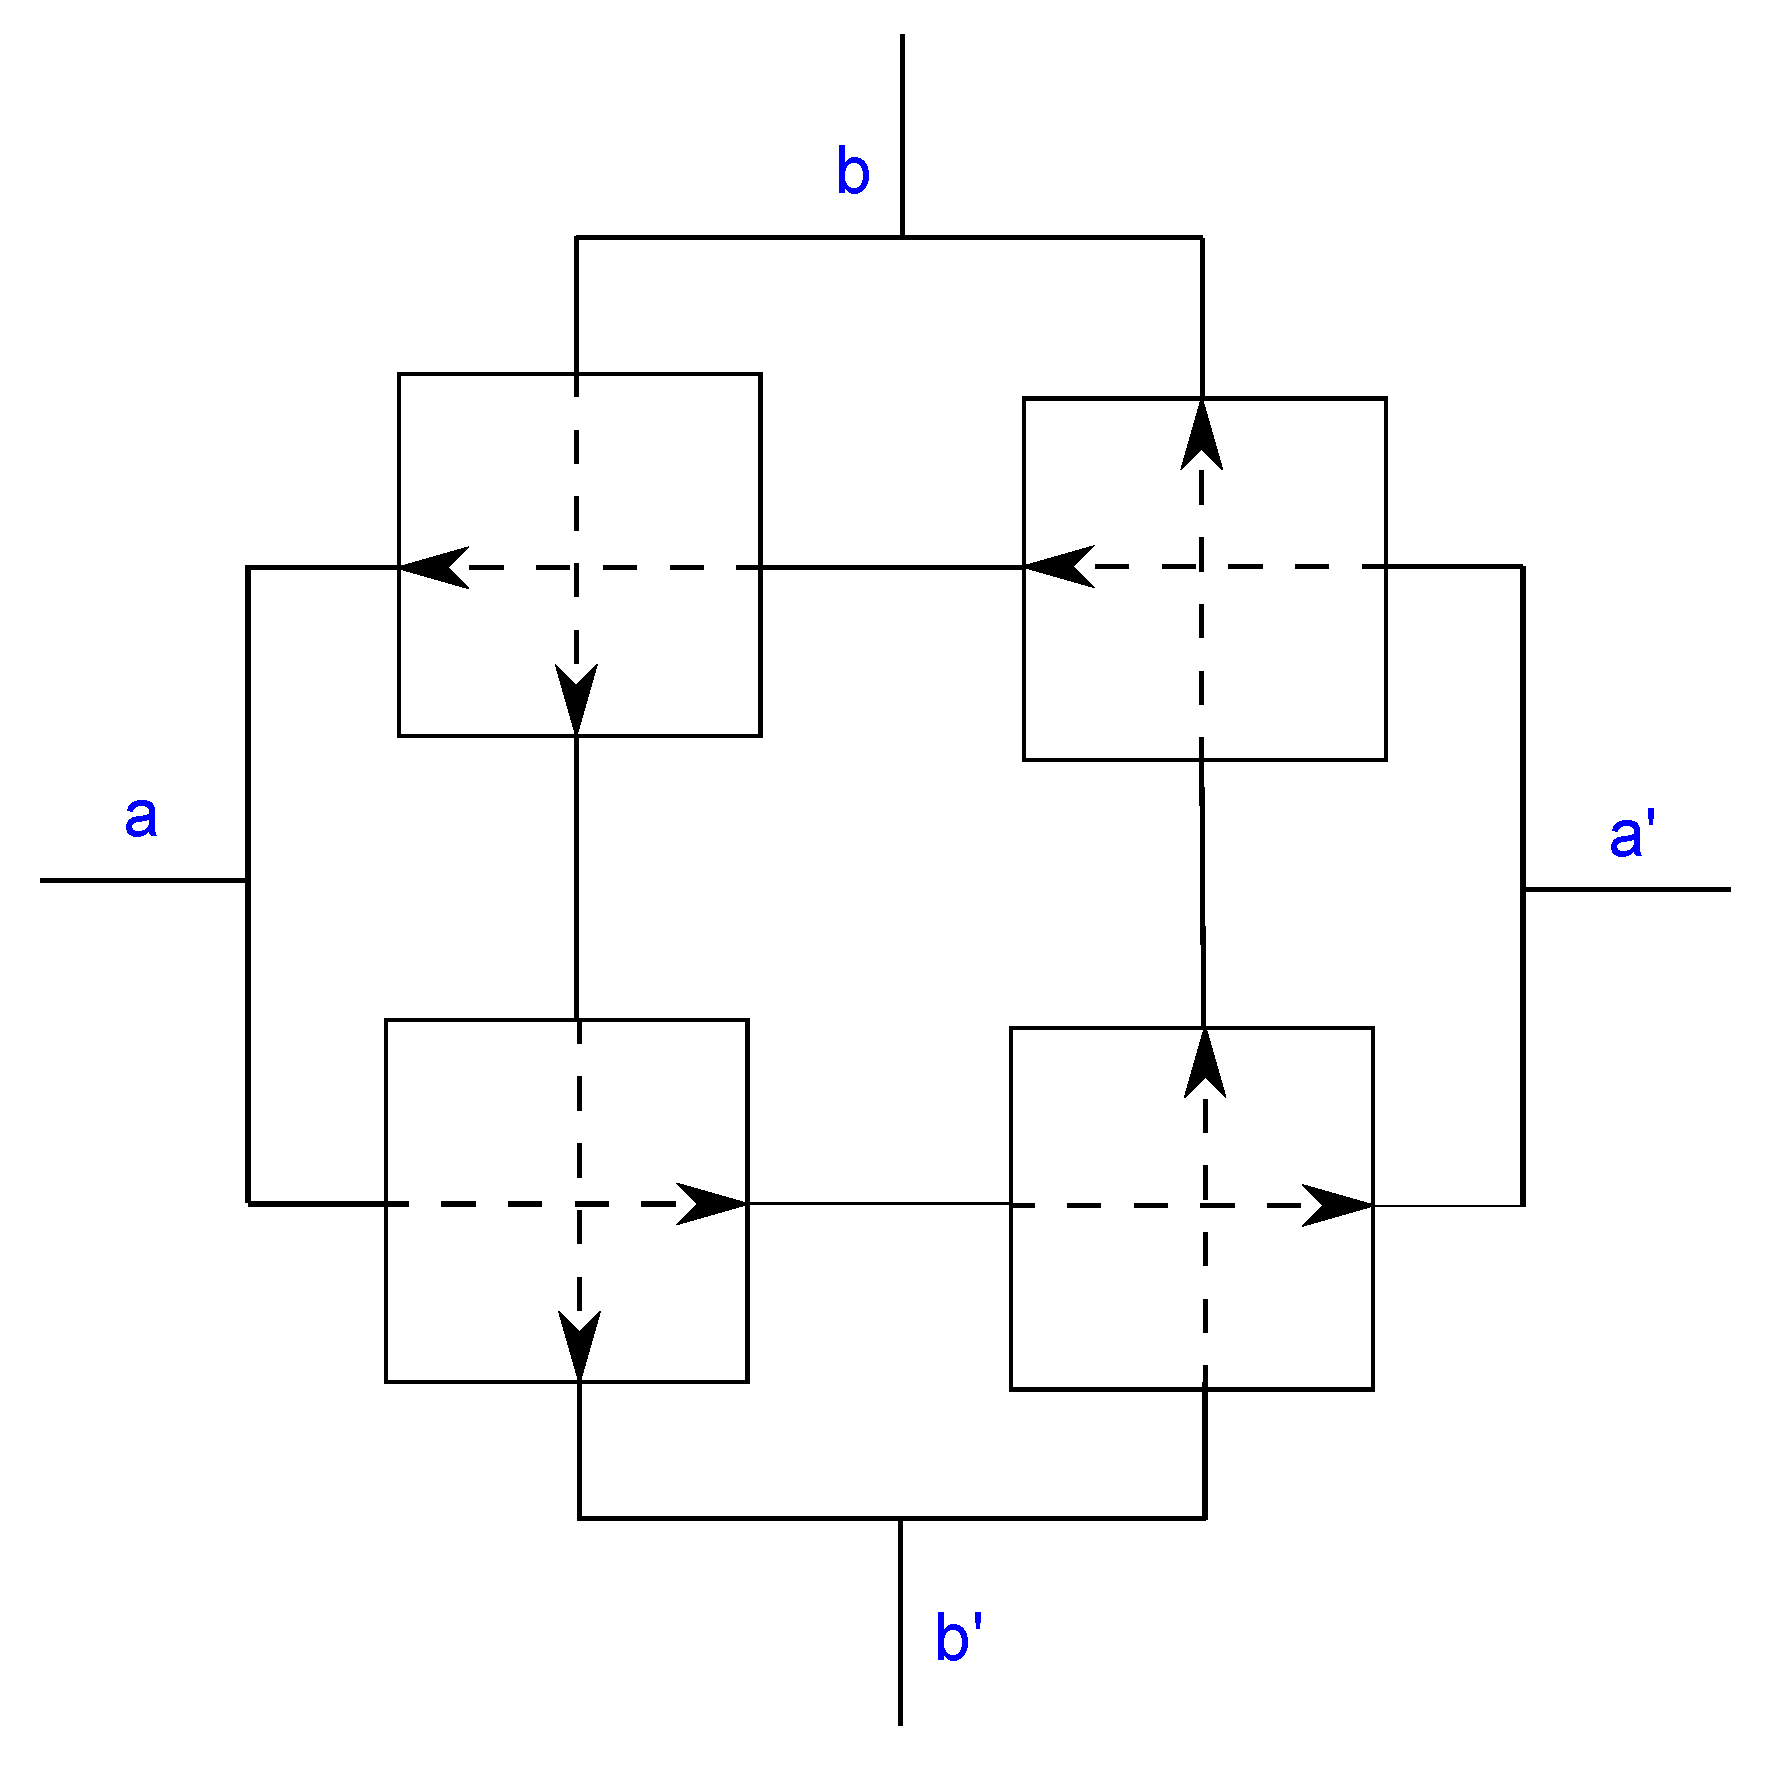
\includegraphics[width=\textwidth]{full_one_use_crossover}
    \caption{A full one use crossover constructed from four directed one use crossovers.}
    \label{full_one_use_crossover}
  \end{subfigure}
  \caption{Composite crossover gadgets}
\end{figure}

\paragraph{In-order Directed Destructive Crossover} This gadget, depicted in Figure~\ref{InOrderCrossover} allows a traversal from $a$ to $a'$, followed by a traversal from $b$ to $b'$.

Initially, no entrance is passable except for $a$, since $V_o$ is passable only in the Verified state, and $S_o$ is
passable only in the Set state. Once the left $V_o \rightarrow V_i$ transition is made, the robot has 2 options.
It can either change the left Set-Verify gadget's state to Set, or leave it as Verified. In either case, the $S_i$
entrance on that toggle is impassable, since a $S_i$ entrance may only be traversed in the Unset state. The
only transition possible on the right crossover is $S_i \rightarrow S_o$, changing the state from Unset to Set.
This completes the first crossing.

Now, there are at most 2 transitions possible: from $a'$ back to $a$, undoing the whole process, or entering at $b$. Note that entering at $b$ is only possible if the left Set-Verify is in the Set state, so let us assume that state change occurred. In that case, the left $S_o \rightarrow S_i$ transition may be performed, changing the left Set-Verify's state to Unset. At that point, the only possible transitions are back to $b$, or through the right Set-Verify's
$V_i \rightarrow V_o$ transition, completing the second crossover.


\paragraph{One Use Directed Crossover} 
The One Use Directed Crossover, depicted in Figure~\ref{OneUseCrossover}, is the gadget needed for our proof. It allows a traversal from $a$ to $a'$ followed by a traversal from $b$ to $b'$, or from $b$ to $b'$ and then $a$ to $a'$.

It is constructed out of an In-order Directed Crossover gadget and a Destructive Directed Crossover, as shown in Figure~\ref{OneUseCrossover}. The $a$ to $a'$ traversal is initially passable, and goes through both gadgets,
blocking the destructive crossover but leaving the in-order crossover open for the $b$ to $b'$ traversal. If the $a$ to $a'$ traversal does not occur, the $b$ to $b'$ traversal is possible via the destructive crossover.

\paragraph{One Use Crossover} 
Four Directed Crossovers can be combined, as shown below, to create a crossover that can be traversed in any direction \cite{Push100}. This is not necessary for our proof but is shown for general interest. Unfortunately, the inability to go through this gadget multiple times in the same direction without first going back through means it likely isn't sufficient for PSPACE-completeness. 

\subsection{3D Push-Pull is NP-hard}
\label{3DNPhard}
In this section we prove that 3D Push-$k$ Pull-$l$ with fixed blocks is NP-hard, for all positive $k$ and $l$. All of the hard work was done in the previous section. Here we will simply show how we can use the additional dimension to tweak the previous gadgets to build them without thin walls. We reduce from 3SAT, constructing our variables from chains of 3D Set-Verify gadgets, and our clauses from the verify side of the corresponding 3D Set-Verify gadget.


\begin{wrapfigure}{r}{0.45\textwidth}
  \centering
%  \begin{figure}[t]
%    \centering
    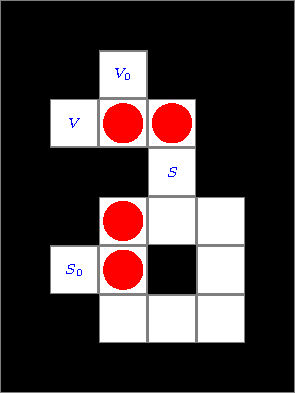
\includegraphics[width=.4\textwidth]{SetVerify3D}
    \caption{A Set-Verify gadget where the entrances and exits extend upward, notated by the diagonal arrows. This gadget is in the unset state.}
    \label{3DSetVerify}
    \vspace{-2mm}
\end{wrapfigure}

\begin{theorem}
3D Push-$k$ Pull-$l$ with fixed blocks is NP-hard, for all positive $k$ and $l$.
\end{theorem}
\begin{proof}
We follow the proof of Theorem~\ref{thm:2DNPhard} using a modified Set-Verify gadget, shown in Figure~\ref{3DSetVerify}. As before, in the unset state the only possible traversal is $S_i$ to $S_0$. This traversal allows the top right bock to be pulled down, moving the gadget into the set state. From here the $V$ to $V_0$ traversal is possible, as well as going back through the $S_0$ to $S$ pathway. However, the $S$ to $S_0$ traversal is not possible. For more detail refer to Section~\ref{sec:SetVerifyGadgets}. We do note that the cyclic ordering of the entrances in the 3D Set-Verify is different from that of the 2D Set-Verify, however this is not important as we no longer need to construct crossovers.

Variables are composed of hallways of 3D Set-Verify gadgets connected $S_0$ to $S$, one for each clause in which the variable appears, as in Figure~\ref{fig:NPVariableGadget}. Clauses are composed of three 3D Set-Verify gadgets connected in parallel as in Figure~\ref{fig:NPClauseGadget}. The details of these constructions follow those in Section~\ref{sec:2DPushPull3SAT} This completes the reduction from 3SAT. In addition, we note that all blocks are in hallways of length at most 3, thus the gadgets still function as described for any positive push and pull values.
\end{proof}




